\documentclass[tikz,dvisvgm,border=0pt]{standalone}
% Shared preamble of the diagrams in vignettes/articles/cuda-kernels.Rmd.
% Render them with `make diagrams` from the package root.
\usepackage[T1]{fontenc}
\usepackage{lmodern}
\usepackage{tikz}
\usetikzlibrary{arrows.meta, positioning, fit, backgrounds, calc, shapes.geometric, decorations.pathreplacing}

\definecolor{host}{HTML}{3B6EA8}
\definecolor{device}{HTML}{2E8B57}
\definecolor{accent}{HTML}{C0571B}
\definecolor{muted}{HTML}{6B6B6B}

% A white card behind every figure, so that it reads in pkgdown's dark mode.
\tikzset{
  every picture/.append style={
    show background rectangle,
    background rectangle/.style={fill=white, rounded corners=6pt},
    inner frame sep=8pt,
    font=\sffamily\small,
    >={Stealth[length=2.2mm]},
  },
  box/.style={draw, rounded corners=3pt, thick, align=center, inner sep=5pt, fill=white},
  hostbox/.style={box, draw=host, fill=host!8},
  devbox/.style={box, draw=device, fill=device!8},
  accbox/.style={box, draw=accent, fill=accent!8},
  region/.style={draw=#1, rounded corners=6pt, thick, dashed, inner sep=8pt},
  heading/.style={font=\sffamily\bfseries\small, text=#1},
  note/.style={font=\sffamily\footnotesize, text=muted, align=center},
  flow/.style={->, thick},
  code/.style={font=\ttfamily\footnotesize},
}

\begin{document}
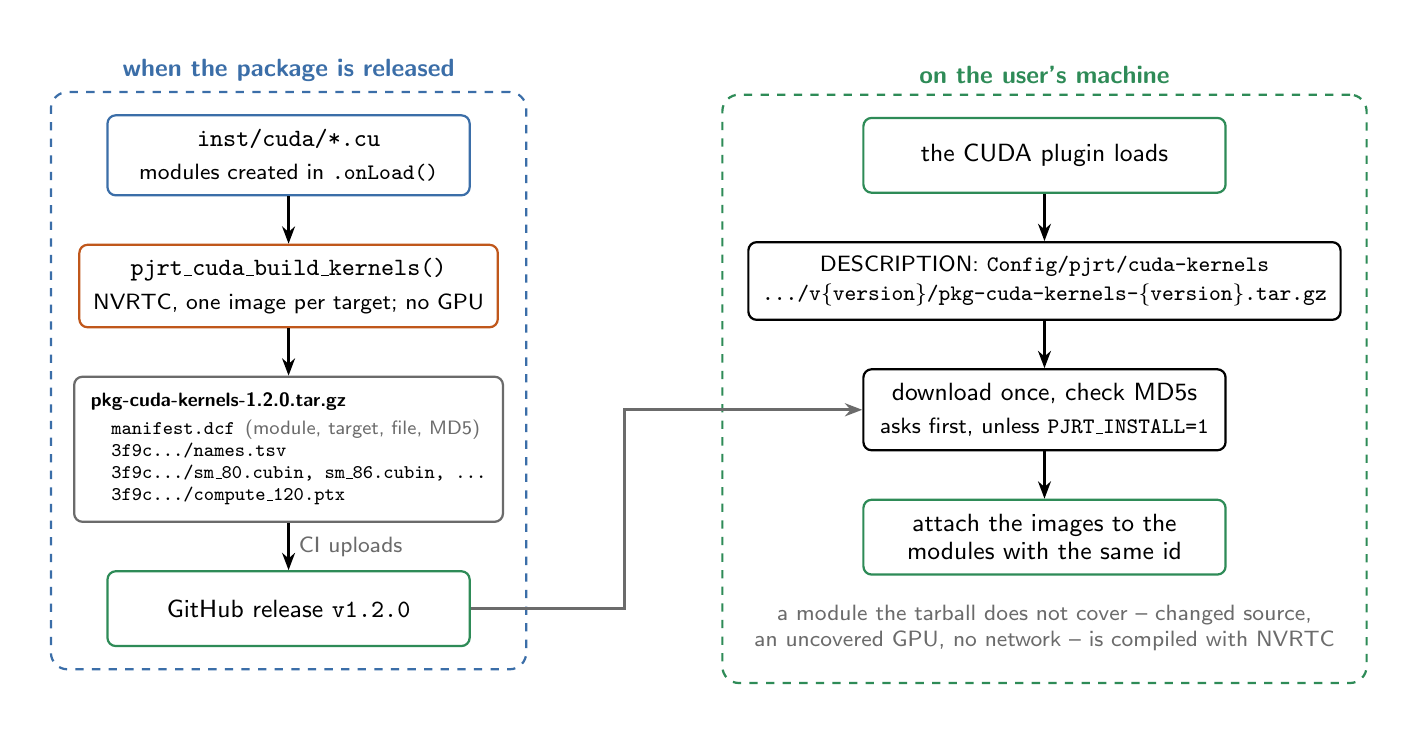
\begin{tikzpicture}[
    stage/.style={box, minimum width=4.6cm, minimum height=0.95cm},
    file/.style={font=\ttfamily\scriptsize, anchor=west, inner sep=1pt},
  ]
  % ---- release time
  \node[hostbox, stage] (src) at (0, 0) {\texttt{inst/cuda/*.cu}\\[1pt]{\footnotesize modules created in \texttt{.onLoad()}}};
  \node[accbox, stage, below=0.6cm of src] (build) {\texttt{pjrt\_cuda\_build\_kernels()}\\[1pt]{\footnotesize NVRTC, one image per target; no GPU}};
  \node[box, draw=muted, anchor=north, align=left, inner sep=6pt, font=\ttfamily\scriptsize] (tar) at ($(build.south) + (0, -0.6)$) {%
    {\sffamily\bfseries pkg-cuda-kernels-1.2.0.tar.gz}\\[2pt]
    \quad manifest.dcf {\sffamily\color{muted}(module, target, file, MD5)}\\
    \quad 3f9c\ldots/names.tsv\\
    \quad 3f9c\ldots/sm\_80.cubin, sm\_86.cubin, \ldots\\
    \quad 3f9c\ldots/compute\_120.ptx};
  \node[devbox, stage, below=0.6cm of tar.south -| build] (rel) {GitHub release \texttt{v1.2.0}};
  \draw[flow] (src) -- (build);
  \draw[flow] (build) -- (build |- tar.north);
  \draw[flow] (build |- tar.south) -- node[right, note] {CI uploads} (rel);
  \node[region=host, fit=(src)(build)(tar)(rel), label={[heading=host]above:when the package is released}] (left) {};

  % ---- user machine
  \node[devbox, stage] (plugin) at (9.6, 0) {the CUDA plugin loads};
  \node[box, stage, below=0.6cm of plugin, font=\sffamily\footnotesize] (url)
    {DESCRIPTION: \texttt{Config/pjrt/cuda-kernels}\\[1pt]{\ttfamily \ldots/v\{version\}/pkg-cuda-kernels-\{version\}.tar.gz}};
  \node[box, stage, below=0.6cm of url] (fetch) {download once, check MD5s\\[1pt]{\footnotesize asks first, unless \texttt{PJRT\_INSTALL=1}}};
  \node[devbox, stage, below=0.6cm of fetch] (attach) {attach the images to the\\[-1pt]modules with the same id};
  \draw[flow] (plugin) -- (url);
  \draw[flow] (url) -- (fetch);
  \draw[flow] (fetch) -- (attach);
  \node[note, below=0.25cm of attach, align=center] (fallback)
    {a module the tarball does not cover -- changed source,\\an uncovered GPU, no network -- is compiled with NVRTC};
  \node[region=device, fit=(plugin)(url)(fetch)(attach)(fallback), label={[heading=device]above:on the user's machine}] (right) {};

  \coordinate (gap) at ($(left.east)!0.5!(right.west)$);
  \draw[flow, very thick, muted] (rel.east) -- (rel.east -| gap) |- (fetch.west);
\end{tikzpicture}
\end{document}
